\chapter{人工データ実験}
\section{シミュレーション}
ニューロン集団のカルシウムイメージングデータをシミュレーションによって作り,解析手法を評価する.
シミュレーションでは1)ニューロンのネットワーク構造を作成し,2)スパイクのシミュレーションを行い,3)蛍光強度の観測データに変換する.
\subsection{ネットワーク構造}
ニューロンのネットワーク構造にはsmall world network\cite{Watts1998}を用いる.
Small world networkはノード数,張り替え確率,初期次数を決めることによってネットワークを作成するアルゴリズムである.
初期次数は,ニューロンが平均何個のニューロンとコネクションを持つかという変数である.
張り替え確率は,初期次数によって作成された規則的なグラフのエッジをランダムに張り替える確率である.
そのため,エッジのうち何割が遠くのニューロンとつながっているかを表す変数である.

ニューロンが他のニューロンとコネクションを持つ状態のことをコネクティビティという.
脳のコネクティビティには,synaptic connectivityとanatomical connectivityとfunctional connectivityの3種類がある.
ネットワーク構造を作成する際に考えているコネクティビティはsynaptic connectivityであり,ニューロンがシナプスを形成してつながっている状態のことである.

実際のニューロンをsmall world networkによって表すために,初期次数と張り替え確率を実データから決める.
今回はこの値はニューロンのコネクションの割合と相互のコネクションの割合から決める.
興奮性ニューロン同士の6.7\%であり,そのうち双方向のコネクションの割合は24\%である\cite{}.
成熟したマウスの抑制性ニューロンと興奮性ニューロンのコネクションの割合は不明だが,興奮性ニューロンから抑制性ニューロンへのコネクティビティと抑制性ニューロンから興奮性ニューロンへのコネクティビティはどちらも78\%であった\cite{Holmgren2003}.
成熟したマウスではより少ないと思われるが,データが見つからなかったため,40\%とした.
相互のコネクションの割合がランダムにエッジを作るよりも高いのは,近いニューロンにコネクションが作られやすいからだと考えられる.
これらのデータを実現するように初期次数と張り替え確率を調整した.
また,抑制性ニューロン同士のコネクティビティは分からないため,興奮性と同じにしている.
\subsection{スパイクシミュレーション}
スパイクのシミュレーションにIzhikevichモデル~\cite{Izhikevich2003}を用いる.
このモデルはHodgikin-Huxleyモデルをもとにしており,計算コストが低い.
このモデルにはニューロンごとに4つのパラメータを設定する必要があり,そのパラメータでニューロンを特徴づける.
本論文では興奮性ニューロンにはregular spiking neurons,抑制性ニューロンにはfast spiking neuronsを用いる.
それらのパラメータを~\Tabref{tab:parameter1}に示す.
ただし,$r_e$と$r_i$は0から1の一様分布に従う確率変数である.

\begin{table}[htb]
  \center
  \begin{tabular}{|c|cccc|} \hline
    ニューロンの種類 & a & b & c & d \\ \hline
    興奮性ニューロン & 0.02 & 0.2 & $-65 + 15 r_e^2$ & $8 - 6r_e^2$ \\
    抑制性ニューロン & $0.02 + 0.08r_i$ & $0.25 - 0.05 r_i$ & -65 & 2 \\ \hline
  \end{tabular}
  \caption{Izhikevichモデルのパラメータ}
  \label{tab:parameter1}
\end{table}

ニューロン間でどれだけシナプス伝達が行われるかも決めなければならない.
これは隣接行列で表すことができる.
隣接行列の$(i,j)$要素は,ニューロン$j$が発火した際にどれくらいの電位がニューロン$j$からニューロン$i$に伝わるかを表す.
興奮性ニューロンからの電位は0から0.5の一様分布からサンプルし,抑制性ニューロンからの電位は-2から0の一様分布からサンプルする.

ニューロンには観測範囲外からの入力がある(以降,外部入力とする).
そのため,シミュレーション中も外部からの電位を乱数としてニューロンの電位に足す.
本論文では,ニューロンの活動も外部入力の大きさで表現する.
活動していない興奮性ニューロンと抑制性ニューロンにはそれぞれ,$\mathcal{N}(0,5)$と$\mathcal{N}(0,2)$に従う乱数を足す.
活動している興奮性ニューロンと抑制性ニューロンにはそれぞれ,$\mathcal{N}(1,5)$と$\mathcal{N}(0.4,2)$に従う乱数を足す.
これらを\Tabref{tab:parameter3}に示す.
活動していないニューロンへの外部入力は\cite{Izhikevich2003}で用いられていたものを採用した.

\begin{table}[htb]
  \center
  \begin{tabular}{|c|cc|} \hline
    ニューロンの種類 & 活動時の外部入力 & 活動していない時の外部入力 \\ \hline
		興奮性ニューロン & $\mathcal{N}(1,5)$ & $\mathcal{N}(0, 5)$ \\
		抑制性ニューロン & $\mathcal{N}(0.4, 2)$ & $\mathcal{N}(0, 2)$ \\ \hline
  \end{tabular}
  \caption{シミュレーションに用いる外部入力の値}
  \label{tab:parameter3}
\end{table}

本論文では同時に活動するニューロンを推定するのが目的の1つである.
ある時間帯にあるニューロングループが活動する時,そのニューロングループには平均値を上げた外部入力を足し,それ以外のニューロンには平均$0$の外部入力を足す.
こうすることで,ニューロングループの活動のみ上がる(つまり蛍光強度が上がる).
実際の脳でもこのように外部からの入力によってニューロンの活動を制御していると考えられる.
あるニューロングループを活動させるには,そのグループのハブとなるニューロンにのみ強い外部入力を与える方法も考えられる.
しかし,ネットワーク構造をかなり工夫しないと実現できないと考えられるため本論文では上記の方法を採用した.

\subsection{カルシウムイメージングモデル}
スパイクデータからカルシウムイオン濃度を計算する~\cite{Vogelstein2009}のモデルを用いる:
\begin{equation}
  [Ca^{2+}]_{i,t} - [Ca^{2+}]_{i,t-1} = - \frac{\Delta}{\tau}([Ca^{2+}]_{i,t-1} - [Ca^{2+}]_b) + An_{i,t} + \sigma_c \sqrt{\Delta} \epsilon_{i,t},
  \label{eq:calcium}
\end{equation}
ただし,$[Ca^{2+}]_{i,t}$をニューロン$i$の時刻$t$でのカルシウムイオン濃度,$[Ca^{2+}]_b$をカルシウムイオン濃度のベースライン,$\Delta$を時間幅,$\tau$は時定数,$A$は1つのスパイクでのカルシウムイオン濃度の上がり幅,$n_{i,t} \in \{0,1\}$はニューロン$i$の時刻$t$でのスパイク,$\sigma_c$はノイズの分散,$\epsilon_{i,t}$は標準正規分布に従う確率変数である.
この人工データではsaturationは考えないこととする.

次に,同論文のモデルを使ってカルシウムイオン濃度$[Ca^{2+}]_{i,t}$をカルシウムイメージングで計測される蛍光強度$F_{i,t}$に変換する:
\begin{equation}
	F_{i,t} = \alpha[Ca^{2+}]_{i,t} + \beta + \sigma_F \epsilon_{i,t},
  \label{eq:intensity}
\end{equation}
$\alpha$は強度,$\beta$はバイアス,$\sigma_F$はノイズの分散である.

\Tabref{tab:parameter2}に使用したパラメータを示す.

\begin{table}[htb]
  \center
  \begin{tabular}{|cccccccc|} \hline
    $[Ca^{2+}]_b$ & $\Delta$ & $\tau$ & $A$ & $\sigma_c$ & $\alpha$ & $\beta$ & $\sigma_F$ \\ \hline
    0.1 & 0.001 & 0.5 & 5.0 & 1.0 & 1.0 & 0 & 1.0 \\ \hline
  \end{tabular}
  \caption{カルシウムイメージングモデルでのパラメータ}
  \label{tab:parameter2}
\end{table}

\subsection{観測モデル}
実データは8 Hzでサンプリングされたデータなので,シミュレーションした蛍光強度を8 Hzで足し合わせる:
\begin{equation}
  x_{i,t'} = \sum_{t=1}^{125} F_{i,t},
  \label{eq:observation}
\end{equation}
ここで,$t'$はサンプリング後の時刻を表す.

\section{結果}
\subsection{設定}
人工データは4種類作成した.
\begin{enumerate}
  \item ニューロンは1つのグループに必ず所属し,近いニューロン同士がグループとなっている
  \item ニューロンは1つのグループに必ず所属し,グループは近さに関係なくランダムに形成される
  \item ニューロンは1つか2つのグループに必ず所属し,同じニューロンが所属しているグループ同士の活動は被らない
\end{enumerate}
800個の興奮性ニューロンと200個の抑制性ニューロンについてシミュレーションを行った.
1つのグループに所属するニューロン数は50〜200個とした.
グループが活動する時間は5sごとに変えた.
シミュレーション時間は470sで,そのうちの10sは安定のため解析から除外した.

\subsection{手法の比較}
Euclidean NMF,logistic regression,glassoの性能の比較を行った.
\textcolor{red}{ここにICAとPCAの結果も加える}
Logistic regressionとglassoについては筆者の卒論を参照されたい.
PCAとICAはNMFと同じく一般化線形成分分析の手法\cite{Cichocki2009}として比較する.

2のタイプについて100種類のデータを生成し,ニューロン同士が同じグループにあるか否かの行列のF1 scoreを比較した.
\begin{figure}[htbp]
    \begin{center}
        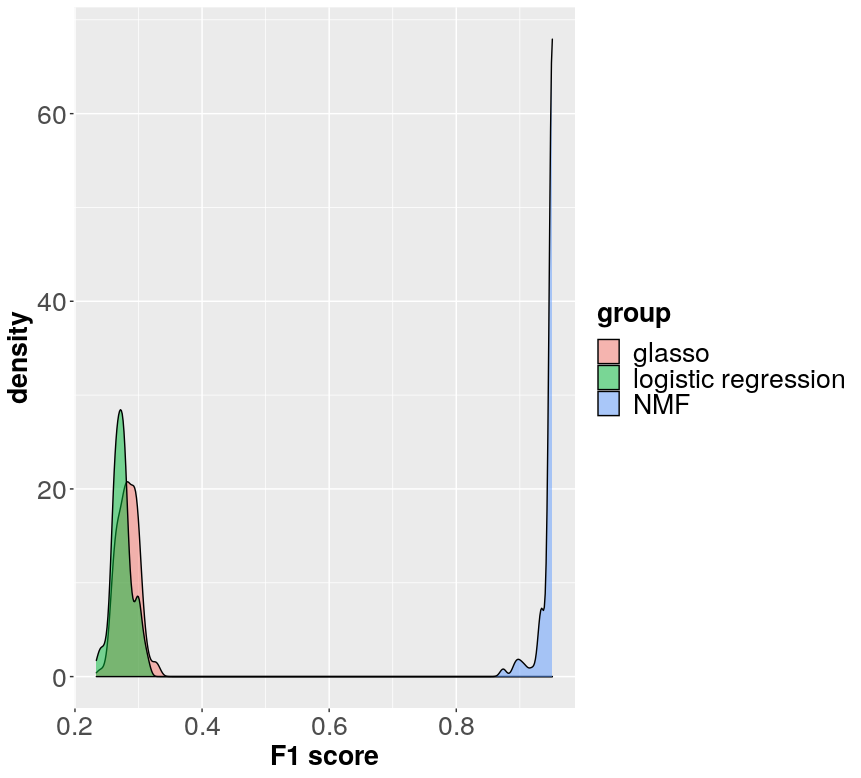
\includegraphics[width=0.5\linewidth]{compare3}
        \caption{NMF,logistic regression,glassoのF1 scoreの密度分布}
        \label{fig:compare3}
    \end{center}
\end{figure}
\Figref{fig:compare3}より,glassoとlogistic regressionの精度は低いことがわかる.
3つの手法のうちNMFがカルシウムイメージングデータを扱うのに適していると考えられる.

\subsection{推定へのネットワーク構造の影響}
グループ推定へのネットワーク構造の影響を調べるために,1と2のネットワーク構造とグループについて100種類のデータを生成し,NMFの推定精度の比較を行った.
人工データは,近いニューロンほどつながりやすい性質をもつので,1の人工データの方がニューロン同士が同期して活動しやすいと思われる.
ここで,2つのニューロンが同期するとは,一方のニューロンが発火してからごく短い間にもう一方のニューロンが発火する状態が続くことである.
実験結果を\Figref{fig:same-exc}~\ref{fig:diff-inh}に示す.\textcolor{red}{もっと綺麗な見せ方にする.検定とかした方がいいのか...?}
\begin{figure}[htbp]
    \begin{center}
        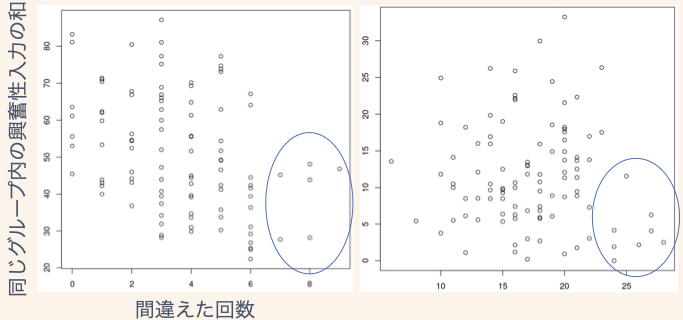
\includegraphics[width=\linewidth]{same-exc}
        \caption{データ1と2について,ニューロンごとの間違えた回数と同じグループからの興奮性入力の和の関係}
        \label{fig:same-exc}
    \end{center}
\end{figure}
\begin{figure}[htbp]
    \begin{center}
      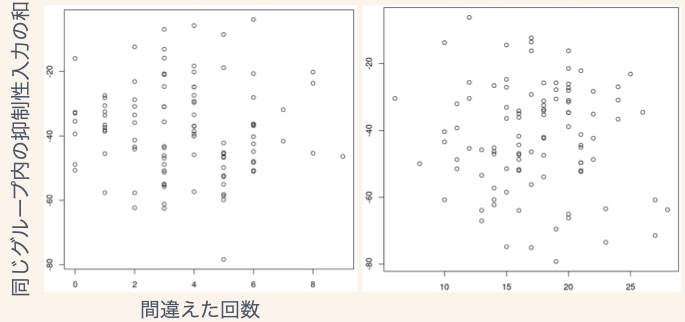
\includegraphics[width=\linewidth]{same-inh}
        \caption{データ1と2について,ニューロンごとの間違えた回数と同じグループからの抑制性入力の和の関係}
        \label{fig:same-inh}
    \end{center}
\end{figure}
\begin{figure}[htbp]
    \begin{center}
        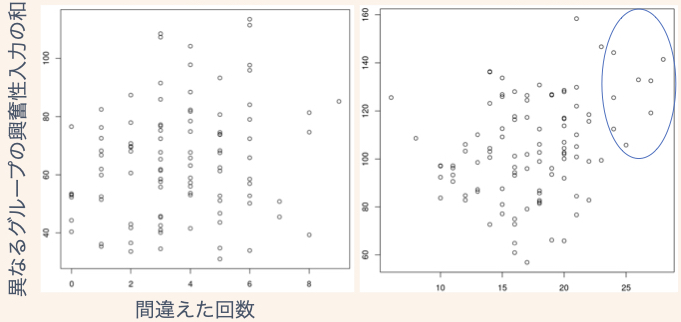
\includegraphics[width=\linewidth]{diff-exc}
        \caption{データ1と2について,ニューロンごとの間違えた回数と異なるグループからの興奮性入力の和の関係}
        \label{fig:diff-exc}
    \end{center}
\end{figure}
\begin{figure}[htbp]
    \begin{center}
        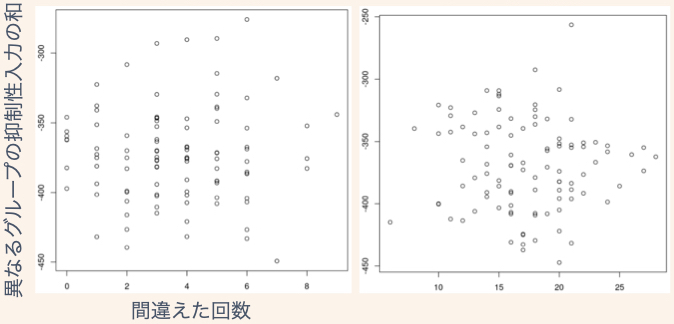
\includegraphics[width=\linewidth]{diff-inh}
        \caption{データ1と2について,ニューロンごとの間違えた回数と異なるグループからの興奮性入力の和の関係}
        \label{fig:diff-inh}
    \end{center}
\end{figure}
\Figref{fig:same-inh},\Figref{fig:diff-inh}より,抑制性の入力は間違える回数には影響しないと思われる.
\Figref{fig:same-exc}より,同じグループからの興奮性入力が小さいと間違えやすいと言える.
\Figref{fig:diff-exc}より,データ2で間違える回数が多かったニューロンは異なるグループからの興奮性入力が大きかった.
データ2ではデータ1よりも近いニューロンが異なるグループに所属する割合が多い.
そのため,異なるグループからの興奮性入力と間違える回数の関係が強く出たと思われる.

他にも推定へのネットワーク構造の影響の調査を試みたが,はっきりとした結果は得られなかった.

\subsection{2グループに所属するとき}
推定精度を出す.
そして被り率も出す.

\subsection{アンサンブルの有用性}
バギングの有用性を確認するために各人工データについて,1回NMFを行った結果,30回初期値を変えた結果,30回ブートストラップした結果のF1 scoreを~\Figref{fig:once-init-boot}に示す.
なお,NMFは20回初期値を変化させて再構成ごさが最小となる結果を1回の結果として用いた.
\begin{figure}[htbp]
    \begin{minipage}{0.5\hsize}
			\begin{center}
					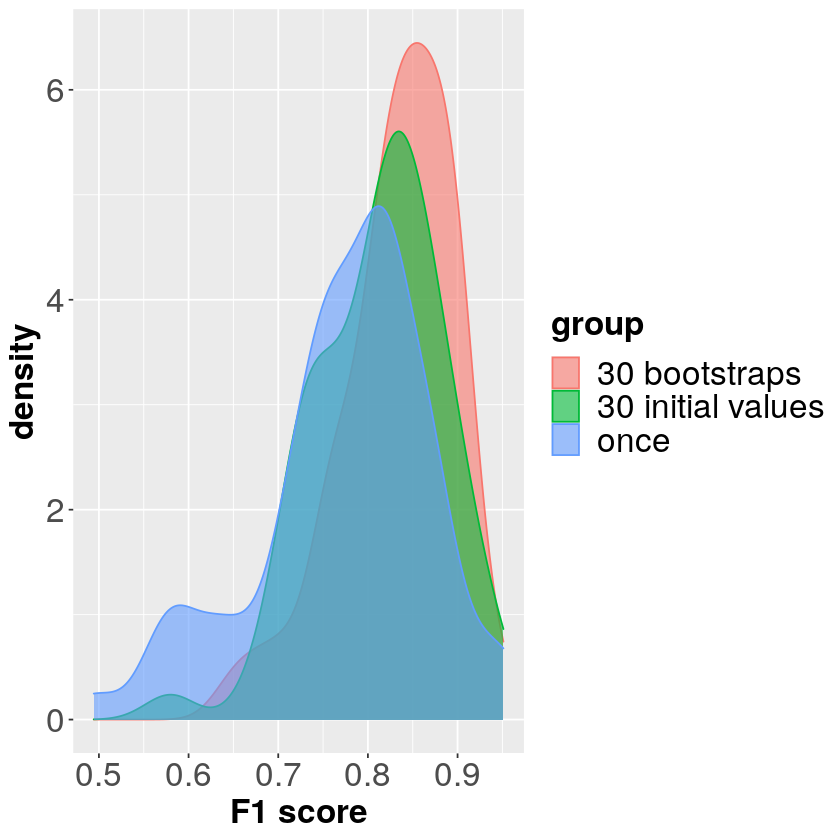
\includegraphics[width=\hsize]{once-init-boot}
					\caption{NMFを1回行った時の$A$,30回初期値を変えた$A$の平均,30回ブートストラップを行った$A$の平均それぞれのF1 scoreの分布.}
					\label{fig:once-init-boot}
			\end{center}
		\end{minipage}
    \begin{minipage}{0.5\hsize}
			\begin{center}
					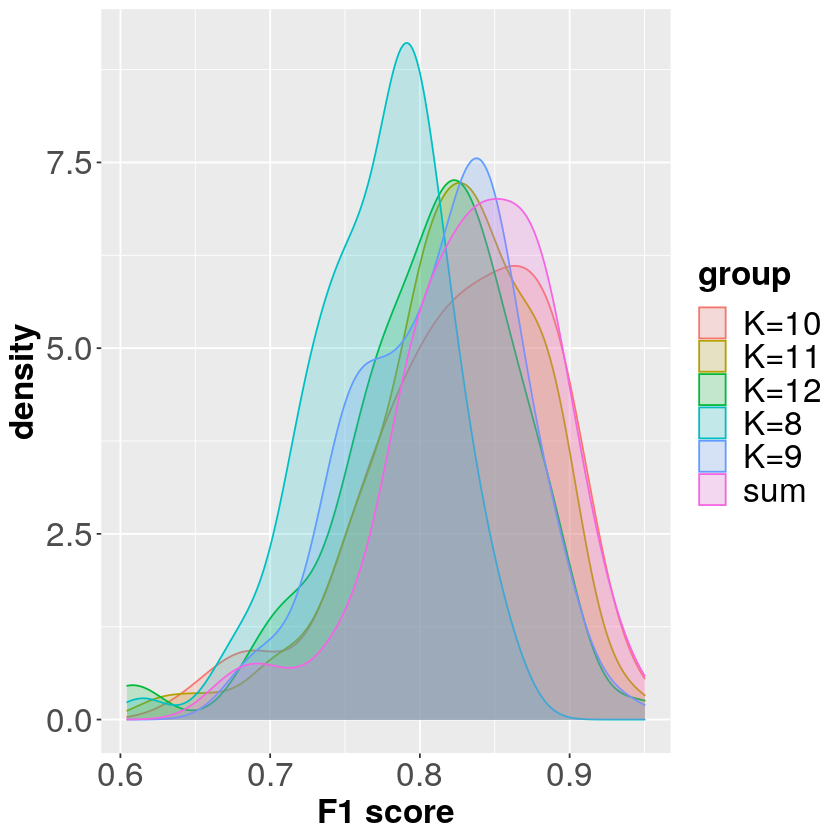
\includegraphics[width=\hsize]{f1all}
					\caption{基底数ごとにブートストラップを行った時の$A$のF1 scoreと全ての$A$の平均をとった時のF1 scoreの分布.}
					\label{fig:f1all}
			\end{center}
		\end{minipage}
\end{figure}
\Figref{fig:once-init-boot}より,ブートストラップを行った方が精度がよくなることがわかる.

基底数別に推定された$A$の平均をとった時のF1 scoreを~\Figref{fig:f1all}に示す.
これより,真の基底数周りの$A$の平均をとることである程度の精度は保たれることがわかる.

\subsection{NMFの基底数}
NMFの基底数を決める方法をいくつか試した.
人工データ86個についてBrunetらとUbrauらの方法で基底数を決めた時に各基底数が何回選ばれるかを~\Figref{fig:cophenetic}.\Figref{fig:uoi}に示す.
Brunetらの方法では真の基底数10に近い基底数が選ばれているが,Ubaruらの方法では小さい基底数が選ばれる傾向にあった.

また,1つの人工データについてAICとAICcを計算した結果を~\Figref{fig:aic},\Figref{fig:aicc}に示す.
どちらも基底数が大きくなるごとに減少する傾向があった.
他の人工データについても同様の結果であった.

\begin{figure}[htbp]
    \begin{minipage}{0.5\hsize}
        \begin{center}
            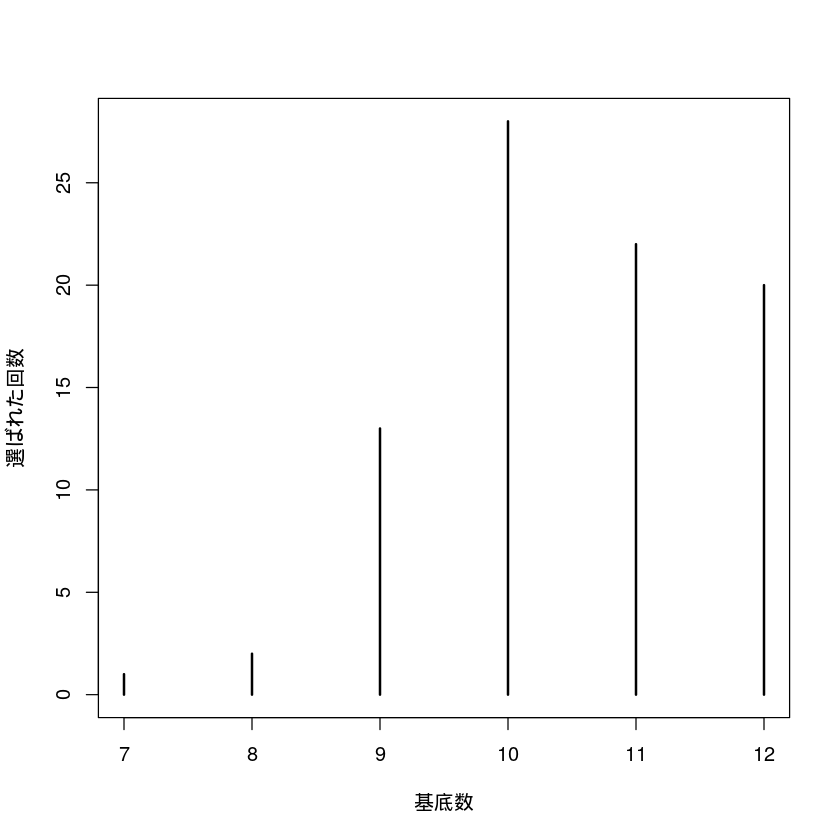
\includegraphics[width=\hsize]{cophenetic}
						\caption{Brunetらの方法で基底数を決めた時に各基底数が選ばれた回数(真の基底数は10).}
            \label{fig:cophenetic}
        \end{center}
    \end{minipage}
    \begin{minipage}{0.5\hsize}
        \begin{center}
            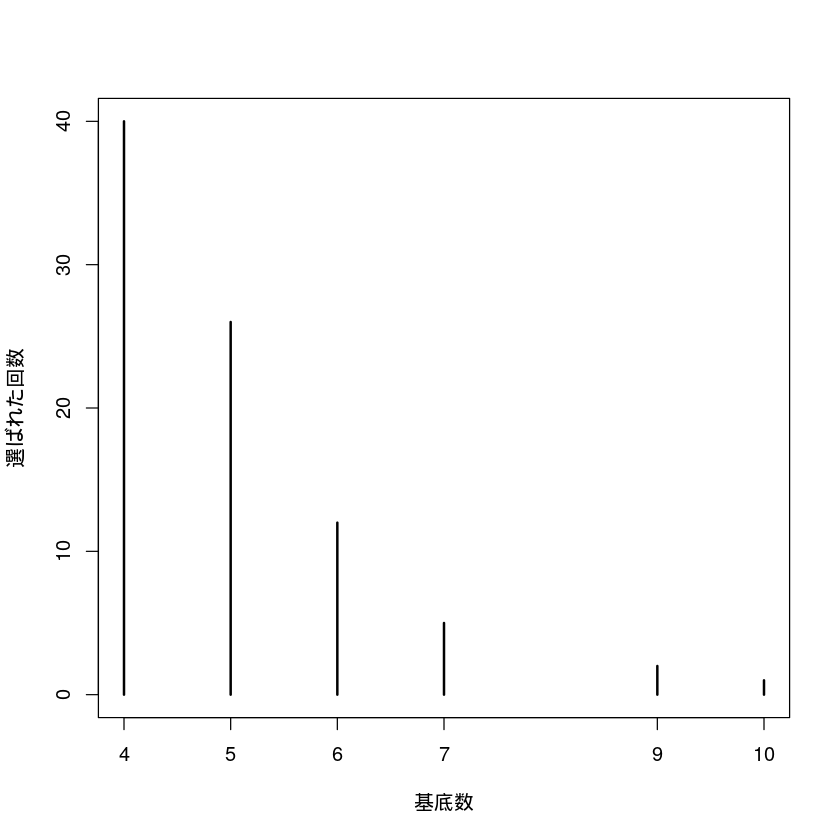
\includegraphics[width=\hsize]{uoi}
						\caption{Ubaruらの方法で基底数を決めた時に各基底数が選ばれた回数(真の基底数は10).}
            \label{fig:uoi}
        \end{center}
    \end{minipage}
\end{figure}
\begin{figure}[htbp]
    \begin{minipage}{0.5\hsize}
        \begin{center}
            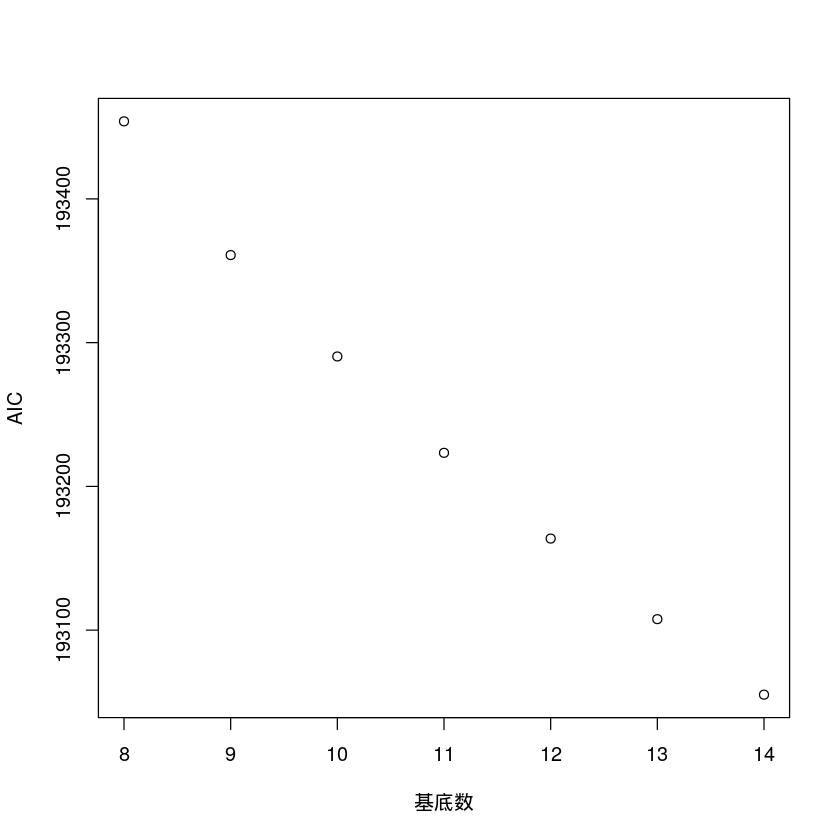
\includegraphics[width=\hsize]{aic}
						\caption{あるデータについてAICを計算した時の結果.}
            \label{fig:aic}
        \end{center}
    \end{minipage}
    \begin{minipage}{0.5\hsize}
        \begin{center}
						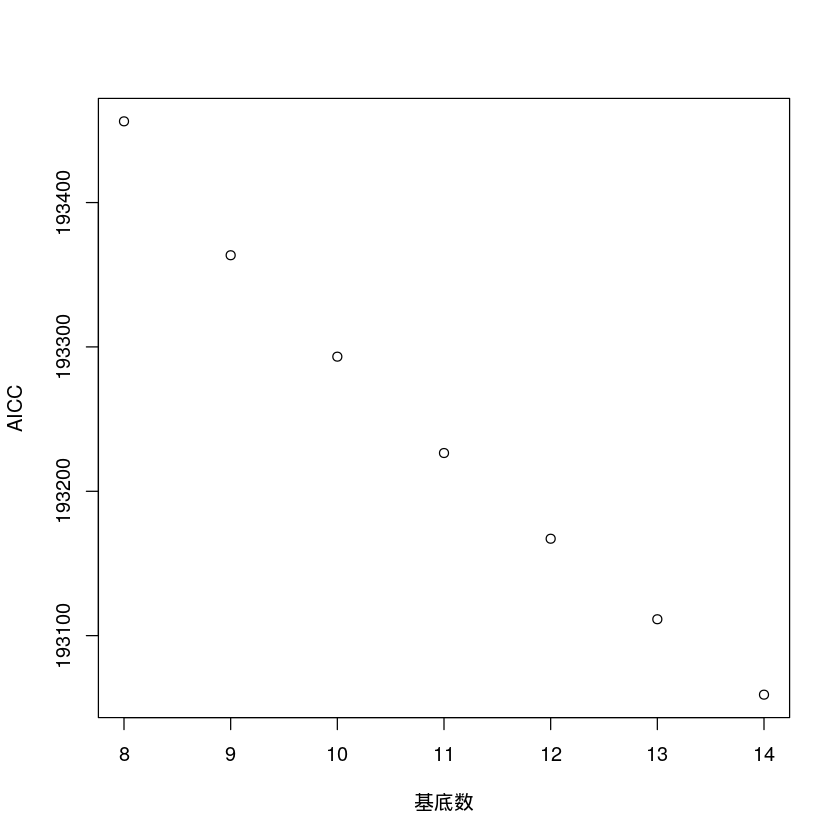
\includegraphics[width=\hsize]{aicc}
						\caption{あるデータについてAICc\cite{Symonds2011}を計算した時の結果.}
            \label{fig:aicc}
        \end{center}
    \end{minipage}
\end{figure}

\subsection{NMFのモデルエビデンス}
